\rhschapter{Object Orienteret Analyse}

\section{Systemdefinition}
\subsection{FACTOR}
\textit{Af Nichlas Bruun}\newline
\textbf{Functionality}
\newline
-Bevægelse af Paddle, Fjernelse af bricks, Scoring, Liv.
\newline
\textbf{Application Domain}
\newline
-Klassisk arkade spil, fokus på kode
og funktionalitet.
\newline
\textbf{Condition}\newline
-Udvikles til Windows styresystemer, baseret på klassisk arkade spil.
\newline
\textbf{Technology}\newline
-Udvikles i Unreal Engine 4, styres med keyboard og har ikke krav
til kraftig PC.
\newline
\textbf{Objects}\newline
-Paddle, Ball, Bricks.
\newline
\textbf{Responsibility}\newline
-Et spilbart produkt.\newline
\newline
Se \cite[chap. 2.7]{Mathiassen200006} for kilde.

\subsection{Sytemdefinition}
\textit{Af Nichlas Bruun}\newline
Unreal Breakout er et klassisk arkade spil, som giver spilleren mulighed for at opleve det klassiske gameplay fra Atari Breakout. Som består af at spilleren bevæger en "paddle" i bunden af skærmen, for at forsøge at holde en bold inden for skærmens rammer, samtidigt med at der skal opnås point ved at fjerne "bricks" i toppen af skærmen.
Der vil være fokus på spillets kode og funktionalitet. Spillet udvikles til Windows PC
i Unreal Engine 4, og styres med keyboard. Spillet vil kunne køre på en Windows PC købt indenfor de sidste 5 år.
Ansvaret over for spilleren vil være et meget basalt virkende spil. \newline \newline
Se \cite[chap. 2.1]{Mathiassen200006} for kilde.
\section{Funktionsliste}
\textit{Af Bjarne Kristensen}\newline
Der er blevet udarbejdet en Funktionsliste (se  tabel \ref{Funktionsliste}) ud fra de funktioner, som er  planlagt at skulle indgå i programmets første version. Disse funktioner er inddelt efter navn, kompleksitet og type. Navnet er hvad funktionen kommer til at omhandle og kompleksitet er hvor udfordrende det vil være at lave den pågældende funktion. Typen er til at bestemme, om det er noget der skal opdateres, læses, sende et signal eller beregne noget. Der er ikke noget komplekst i spillet, der er to funktioner som menes at have en kompleksitet på medium, dette relatere til boldens interaktion med andre objekter. De resterende funktioner menes at være simple at implementere.\newline
\newline
Se \cite[chap. 7.3, fig. 7.6]{Mathiassen200006} for kilde.

\begin{table}[]
\centering
\caption{Funktionsliste}
\label{Funktionsliste}
\begin{tabular}{|l|l|l|}
\hline
\multicolumn{1}{|c|}{Navn} & \multicolumn{1}{c|}{Kompleksitet} & \multicolumn{1}{c|}{Type} \\ \hline
Start Game & simpel & update \\ \hline
Exit Menu & simpel & update \\ \hline
Exit Game & simpel & update \\ \hline
Release Ball & medium & update / compute \\ \hline
Bounce Ball & medium & update / compute \\ \hline
Move Paddle & simpel & update / compute \\ \hline
Break Brick & simpel & update \\ \hline
Change Score & simpel & update / compute \\ \hline
Show Score & simpel & read \\ \hline
\end{tabular}
\end{table}

\section{Analysediagram}
\textit{Af Nichlas Bruun}\newline
\begin{figure}
	\begin{center}
		\caption{Analysediagram.}
		\label{dia:analysediagram}
		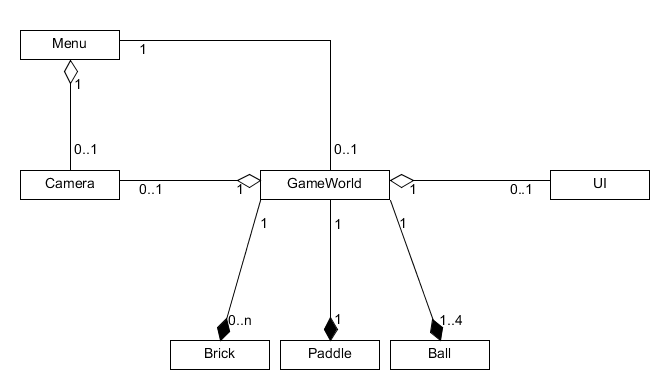
\includegraphics[width=1.0\linewidth]{pictures/ooa/analysediagram}
	\end{center}
\end{figure}
\subsection{Menu}
Menu klassen kommer til at være et "level blueprint" i Unreal Engine. Den skal håndtere indlæsning af menupunkter, i form af knapper og baggrundsgrafik. Menuens blueprint kommer til at håndtere "OnClick events" hvilket i dette tilfælde er en "Play-" og en "Quit-knap". Som i samme nævnte rækkefølge, kommer til at starte spillet, og lukke spillet.

\subsection{Camera}
Camera håndtere spillets synspunkt, altså hvad spilleren kan se. Kameraet kan vælge ikke at vise spilleren nogle objekter, som der muligvis har været behov for under udviklingen af spillet. Kameraet kan beskrives som en support klasse, da den ikke direkte ændre på nogle elementer, men bare viser eller ikke viser dem. Samme blueprint vil være brugt både på kameraet i menuen, og kameraet i selve spillet.

\subsection{GameWorld}
GameWorld vil ligesom Menu-klassen, være et "level blueprint". GameWorld kommer til at være roden til alt spillets logik, og skal bl.a. indlæse alle spillets elementer når spillet startes, og når spillet skifter bane. Klassen kommer også til at lave funktionskald til de andre klasser der er relevant i spillet f.eks. Brick og Paddle.

\subsection{UI}
UI-klassen vil holde styr på at vise og opdatere brugergrænsefladen i spillet. 
Som i dette tilfælde vil være at vise og opdatere spillerens point og liv.

\subsection{Brick}
Brick-klassen kommer til at ligge på alle de objekter spilleren skal forsøge at ramme med bolden. Klassen vil håndtere at når bolden kollidere med en "Brick" vil denne Brick forsvinde, og der vil blive lavet de korrekte funktionskald til at opdatere spillerens score, alt efter hvilken type af Brick bolden rammer.

\subsection{Paddle}
Paddle-klassen kan tolkes som selve spillerens klasse, denne klasse vil håndtere input fra spilleren. Det vil sige at når spilleren trykker på venstre eller højre pil, bevæger Paddlen sig i den korrekte retning. Den vil også give de korrekte funktionskald til bolden, alt efter hvilken del af Paddlen bolden rammer, og give den korrekte vinkel med til bolden. Når spillet startes eller når spilleren dør, Vil Paddlen også kunne bruges til at skyde bolden afsted, da bolden er stationær på Paddlen i begyndelsen. Bolden skydes afsted fra paddlen ved brug af mellemrumstasten. 

\subsection{Ball}
Ball er bolden i spillet, og klassen vil håndtere bolden, samtidigt med de tidligere nævnte funktionskald. Bolden vil også stå for vind/tab-konditionen i spillet, ved at tjekke om den er udenfor bunden af skærmen, og lade spilleren miste liv hvis den er udenfor.\newline
\newline
Se \cite[chap. 4]{Mathiassen200006} for kilde.


\section{Hændelsestabel}
\textit{Af Bjarne Kristensen}\newline
En hændelse, i objektorienteret kontekst, er en situation hvor en eller flere objekter er involveret. Det er f.eks. hændelser hvor spilleren giver et input som objekter i spillet skal agere på. Det kan også være hændelser i spillet som sker når to objekter kolliderer med hinanden og en aktion ønskes. I tabel \ref{eventtabel} er der opstillet hvilke hændelser vi regner med vil ske, og hvilke objekter der kan være involveret i disse hændelser.\newline
\newline
Se \cite[chap. 3]{Mathiassen200006} for kilde.
\begin{table}[]
\centering
\caption{Hændelsestabel}
\label{eventtabel}
\begin{tabular}{|l|c|c|c|c|c|c|c|}
\hline
Events/Klasser & Paddle & Ball & Brick & Menu & Gameworld & Camera & UI \\ \hline
Player clicks on menu obj &  &  &  & X &  &  &  \\ \hline
Player moves paddle & X &  &  &  & X &  &  \\ \hline
Player releases ball & X & X &  &  & X &  &  \\ \hline
Ball collides with object & X & X & X &  & X &  &  \\ \hline
Score updates &  & X & X &  & X &  & X \\ \hline
\end{tabular}
\end{table}

\section{Use Cases}
\textit{Af Mathias Forsberg}\newline
\textbf{Start Spillet}\newline

\textbf{Scope:}\newline
I menuen.\newline

\textbf{Description:} \newline
Spilleren trykker på \textit{play}-knappen med musen, i menuen for at komme til \textit{gameworld}. \newline

\textbf{Preconditions:}\newline
Spilleren skal befinde sig i menuen for at use casen kan startes.\newline

\textbf{Success Guarantee:}\newline
Når use casen er opfyldt vil spillet gå fra menuen til \textit{gameworld}.\newline

\textbf{Main Success Scenario:}\newline
Spilleren befinder sig i menuen og klikker med musen på \textit{play}-knappen og \textit{gameworld} vises frem på skærmen.\newline

\textbf{Extensions:}\newline
Befinder spilleren sig allerede i \textit{gameworld} vil det ikke være muligt at trykke på \textit{play}-knappen da den ikke er vises i \textit{gameworld}.\newline \newline



\textbf{Luk Spillet}\newline

\textbf{Scope:}\newline
I menuen. \newline

\textbf{Description:} \newline
Spilleren kan lukke spillet ved at trykke på \textit{exit}-knappen med musen.\newline

\textbf{Preconditions:}\newline
Spilleren skal befinde sig i menuen for at use casen kan startes.\newline

\textbf{Success Guarantee:}\newline
Når use casen er opfyldt vil spillet blive lukket. \newline

\textbf{Main Success Scenario:}\newline
Spilleren befinder sig i menuen og klikker på \textit{exit}-knappen med musen, hvorefter spillet vil lukke.\newline

\textbf{Extensions:}\newline
Befinder spilleren sig i \textit{gameworld} vil \textit{exit}-knappen ikke være vist og spilleren kan derfor ikke interagere med den. \newline \newline


\textbf{Bevægelse af Paddle}\newline

\textbf{Scope:}\newline
I \textit{Gameworld}.\newline

\textbf{Description:} \newline
Spilleren kan ved hjælp af højre og venstre piletast bevæge \textit{Paddlen} til henholdsvis højre og venstre.\newline

\textbf{Preconditions:}\newline
Spilleren har startet spillet igennem menuen.\newline

\textbf{Success Guarantee:}\newline
Bliver use casen opfyldt korrekt vil \textit{Paddlen} blive bevæget til siderne i takt med at spilleren trykker piletasterne ned.\newline

\textbf{Main Success Scenario:}\newline
 a. Spilleren trykker højre piletast ned og \textit{Paddlen} bevæger sig til højre.\newline
 b. Spilleren trykker venstre piletast ned og \textit{Paddlen} bevæger sig til venstre.\newline \newline


\textbf{Skyd}\newline

\textbf{Scope:}\newline
I \textit{Gameworld}.\newline

\textbf{Description:} \newline
Bolden skydes fra \textit{Paddlen} ved brug af \textit{space}-knappen, dette kan kun gøres når spillet startes eller efter bolden har været uden for spilbanen. \newline

\textbf{Preconditions:}\newline
Spilleren har startet spillet igennem menuen og har ikke skudt endnu, eller bolden har lige været udenfor spilbanen.\newline

\textbf{Success Guarantee:}\newline
Bliver use casen opfyldt korrekt vil bolden blive skudt fra \textit{Paddlen}.\newline

\textbf{Main Success Scenario:}\newline
Spilleren har startet spillet og bolden er stadig placeret på \textit{Paddlen}, eller bolden har lige været uden for spilbanen. spilleren trykker på \textit{space}-knappen og bolden bliver skudt fra \textit{Paddlen}.\newline

\textbf{Extensions:}\newline
Bolden er blevet skudt fra \textit{Paddlen} og har ikke været udenfor spilbanen og kan derfor ikke blive skudt fra \textit{Paddlen} igen da den ikke er placeret der.\newline \newline


\textbf{Gå tilbage til menuen}\newline

\textbf{Scope:}\newline
I \textit{Gameworld}.\newline

\textbf{Description:} \newline
Spilleren går tilbage til menuen fra \textit{gameworld} ved at trykke på \textit{escape}-knappen.\newline

\textbf{Preconditions:}\newline
Spilleren har startet spillet og befinder sig i \textit{gameworld}.\newline

\textbf{Success Guarantee:}\newline
Bliver use casen opfyldt korrekt vil spilleren blive vist menuen igen og \textit{gameworld} vil lukke.\newline

\textbf{Main Success Scenario:}\newline
Spilleren har startet spillet og trykker på \textit{escape}-knappen, herefter vil menuen blive vist og \textit{gameworld} vil stoppe. \newline

\textbf{Extensions:}\newline
Befinder spilleren sig allerede i menuen vil \textit{escape}-knappen ikke have nogen effekt.\newline
\newline
Se \cite[chap. 6.1]{Mathiassen200006} for kilde.